This system is divided in two PCBs, one of the PCBs is called the Main DCM wich as the capacitor and is the PCB that has the headers to provide power supply to the low voltage system. The other PCB is called the DCM 2, and has one connector to connect to the Main DCM. This situation is illustrated in the the following Figures.
\begin{figure}[!htb]
\centering
  \begin{subfigmatrix}{2}
    \subfigure[Top Layer.]{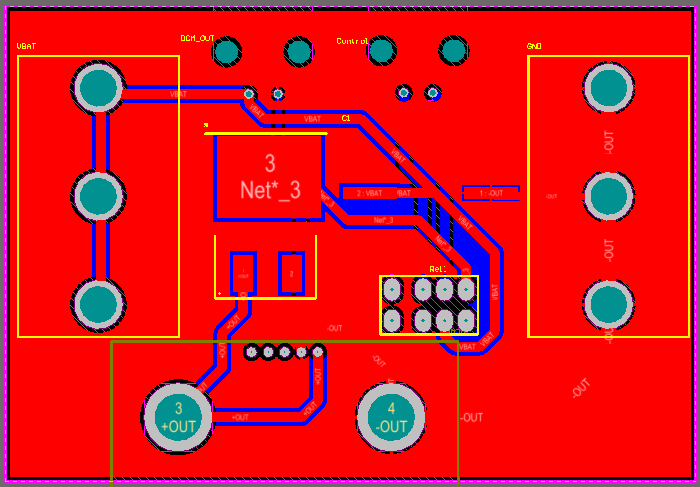
\includegraphics[width=0.4\linewidth]{Figures/2D_Layout_TOP_DCM1.PNG}}
    \subfigure[Bottom Layer.]{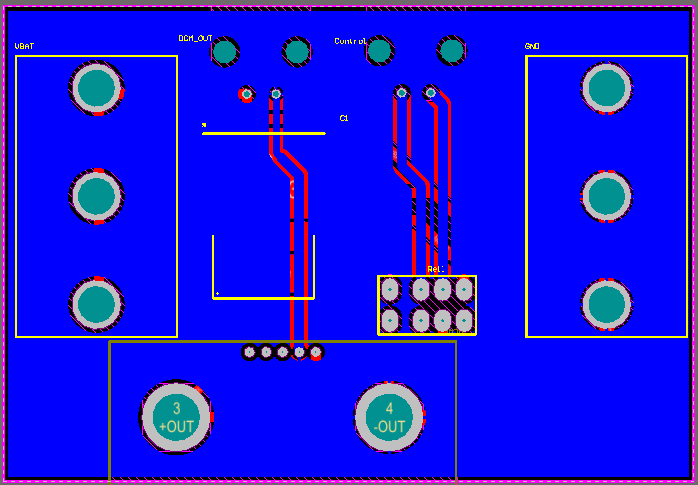
\includegraphics[width=0.4\linewidth]{Figures/2D_Layout_BOT_DCM1.PNG}}
  \end{subfigmatrix}
  \caption{Layout of the DCM main PCB.}
  \label{fig:DCM1Layout}
\end{figure}

\begin{figure}[!htb]
	\centering
	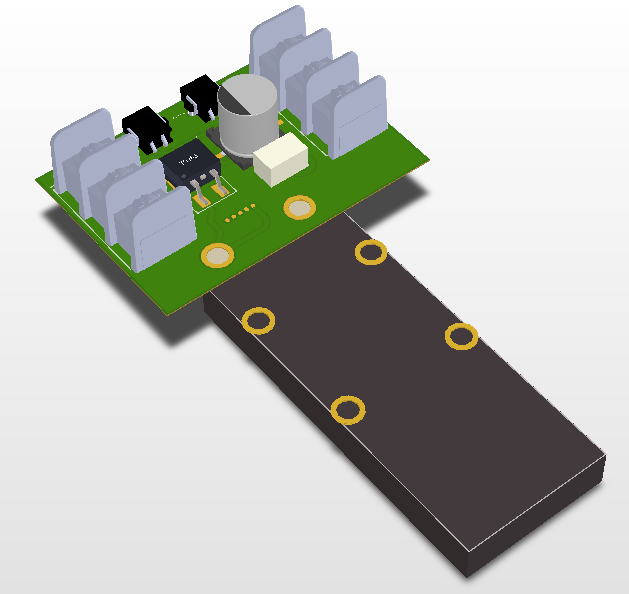
\includegraphics[width=0.5\linewidth]{Figures/3D_Layout_Front.PNG}
	\caption{3D view of DCM main PCB.}
	\label{fig:DCM1Layout3D}
\end{figure}

\begin{figure}[!htb]
	\centering
	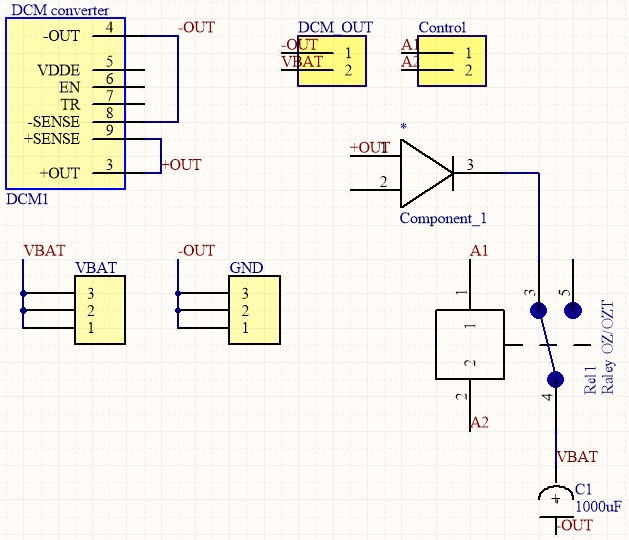
\includegraphics[width=0.5\linewidth]{Figures/Schematic_DCM_MAIN.PNG}
	\caption{Schematic of the DCM Main PCB.}
	\label{fig:DCM1Schematic}
\end{figure}

\textbf{DCM 2 PCB}
\begin{figure}[!htb]
\centering
  \begin{subfigmatrix}{2}
    \subfigure[Top Layer.]{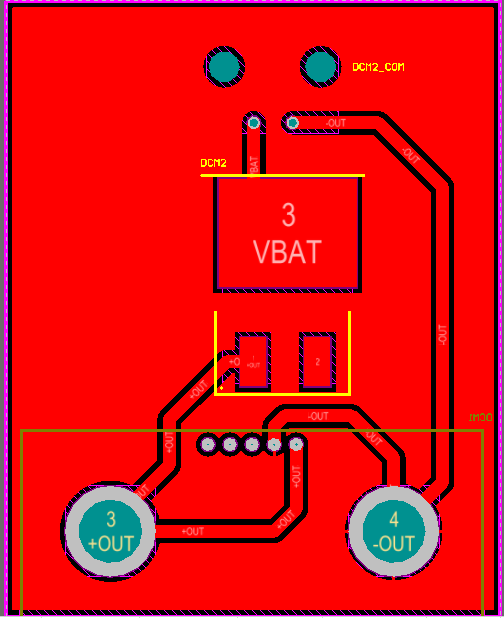
\includegraphics[width=0.3\linewidth]{Figures/2D_Layout_TOP_DCM2.PNG}}
    \subfigure[3D view of DCM 2 PCB.]{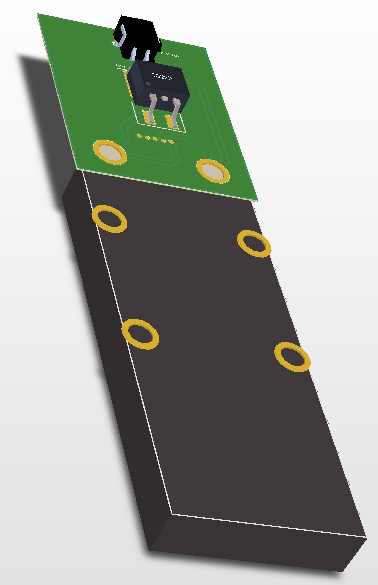
\includegraphics[width=0.3\linewidth]{Figures/3D_Layout_Front_DCM2.PNG}}
  \end{subfigmatrix}
  \caption{Layout of the DCM 2 PCB.}
  \label{fig:DCM2Layout}
\end{figure}
\newline

\begin{figure}[!htb]
	\centering
	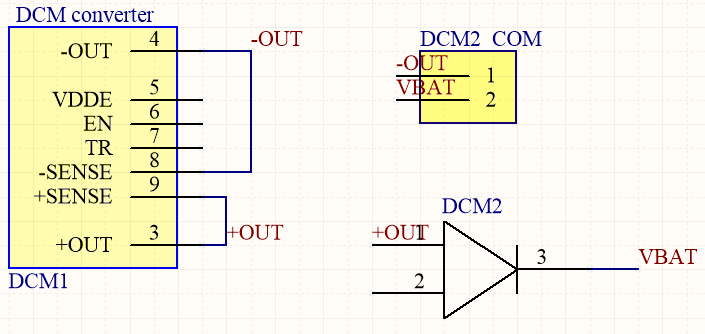
\includegraphics[width=0.5\linewidth]{Figures/DCM2_Schematic.PNG}
	\caption{Schematic of the DCM 2 PCB.}
	\label{fig:DCM2Schematic}
\end{figure}